\documentclass[default]{beamer}
\setbeamertemplate{navigation symbols}{}

\usetheme{CambridgeUS}
\useoutertheme{infolines}
\useinnertheme{circles}
\usecolortheme{seahorse}

\usepackage{cmap}							% Поддержка поиска русских слов в PDF (pdflatex)
\usepackage[T2A]{fontenc}       			%поддержка кириллицы
\usepackage[utf8]{inputenc}					% Выбор языка и кодировки
\usepackage[english, russian]{babel}
\usepackage{csquotes}
\usepackage{tikz}
\usepackage{textcomp}
\usepackage{textpos}
\usepackage{calc}

\usetikzlibrary{calc}

\usepackage[
	language=auto,
	autolang=other,
	backend=biber,
	style=authortitle,
	sorting=ydnt
]{biblatex}
\addbibresource{common-cog.bib}
				
\DeclareSourcemap{
	\maps[datatype=bibtex, overwrite]{
		\map{
			\step[fieldset=langid, fieldvalue=english]
			\step[fieldset=doi, null]
			\step[fieldset=issn, null]
			\step[fieldset=isbn, null]
			\step[fieldset=url, null]
			\step[fieldsource=language, fieldset=langid, origfieldval]
		}
	}
}


\graphicspath{{../../images/}} 			% Пути к изображениям

\makeatletter
\setbeamertemplate{footline}
{
	\leavevmode%
	\hbox{%
		\begin{beamercolorbox}[wd=.333333\paperwidth,ht=2.25ex,dp=1ex,center]{author
				in head/foot}%
			\usebeamerfont{author in
				head/foot}\insertshortauthor~~\beamer@ifempty{\insertshortinstitute}{}{(\insertshortinstitute)}
		\end{beamercolorbox}%
		\begin{beamercolorbox}[wd=.333333\paperwidth,ht=2.25ex,dp=1ex,center]{title in
				head/foot}%
			\usebeamerfont{title in head/foot}\insertshorttitle
		\end{beamercolorbox}%
		\begin{beamercolorbox}[wd=.333333\paperwidth,ht=2.25ex,dp=1ex,right]{date in
				head/foot}%
			\usebeamerfont{date in head/foot}\insertshortdate{}\hspace*{2em}
			\insertframenumber{}\hspace*{2ex} 
		\end{beamercolorbox}
	}%
	\vskip0pt%
}

\addtobeamertemplate{frametitle}{}{
	\begin{textblock*}{100mm}(\textwidth-10pt,-25pt)
		
\includegraphics[height=0.8cm]{advert/hse.png}
	\end{textblock*}
}

\renewcommand*{\bibfont}{\footnotesize}
\newenvironment{proenv}{\only{\setbeamercolor{local structure}{fg=green}}}{}
\newenvironment{conenv}{\only{\setbeamercolor{local structure}{fg=red}}}{}

\begin{document}
	
	\title[ИПиКА]{Интеллектуальное планирование и когнитивные архитектуры}
	\author[Панов,Яковлев]{Константин Яковлев, Александр Панов}
	\institute[ВШЭ]{Базовая кафедра <<Математические методы системного анализа>> Института системного анализа РАН\\
	\url{www.cs.hse.ru/mmsa}\\
	Федеральный исследовательский центр <<Информатика и управление>>\\Российской академии наук}
	\date{18 апреля 2016~г.} 
	
	\begin{frame}
		\titlepage
	\end{frame}

	\begin{frame}
		
		
\includegraphics[width=\textwidth]{advert/slide2.jpg}
	\end{frame}
	
	\begin{frame}
		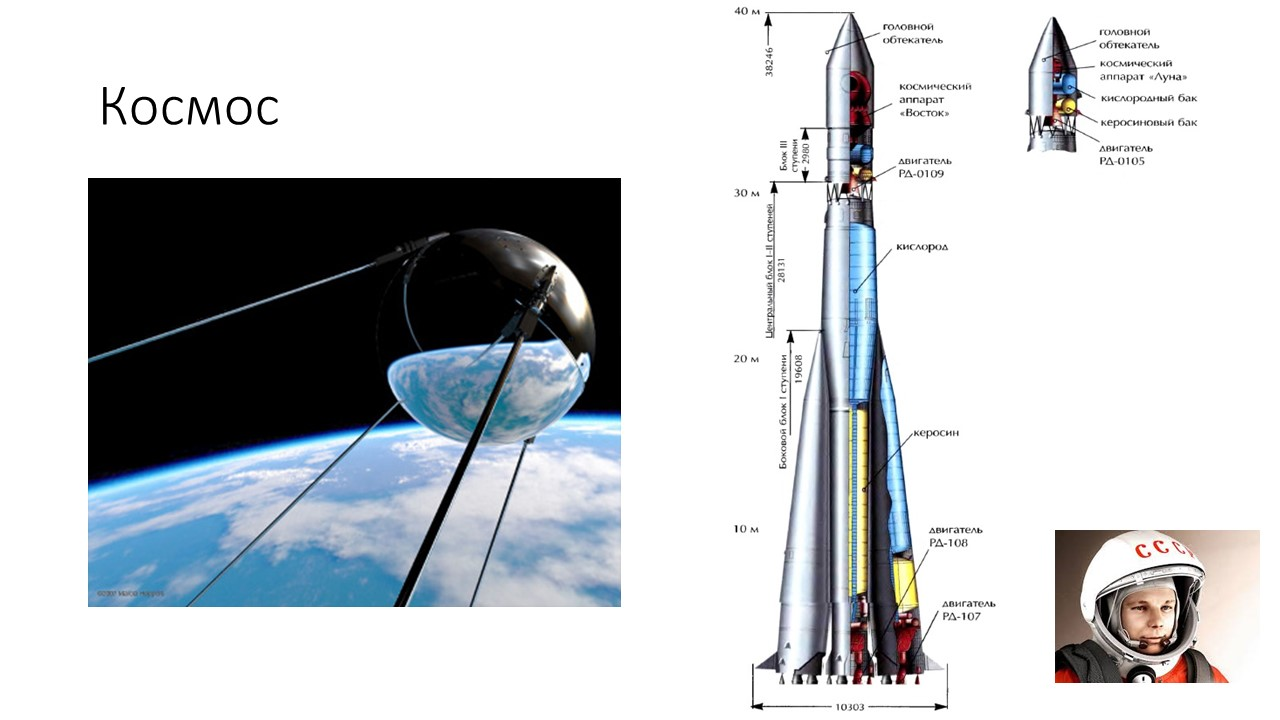
\includegraphics[width=\textwidth]{advert/slide3.jpg}		
	\end{frame}

	\begin{frame}
		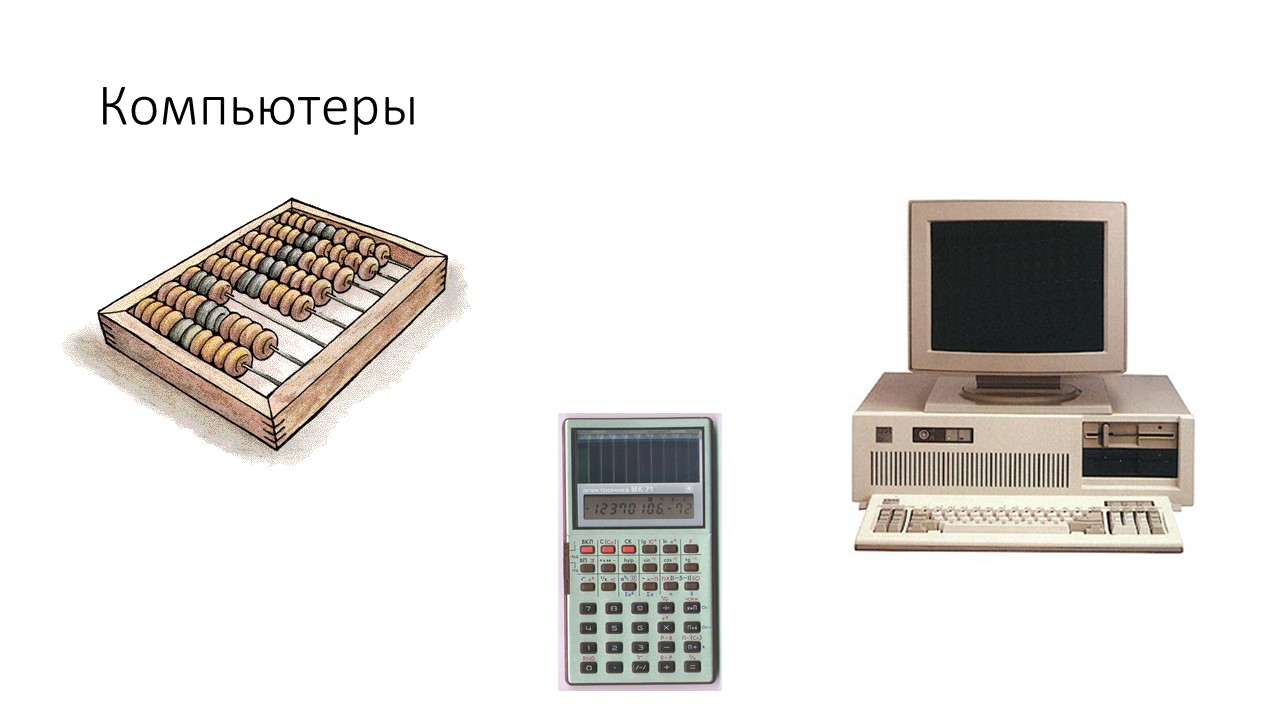
\includegraphics[width=\textwidth]{advert/slide4.jpg}
	\end{frame}

	\begin{frame}
		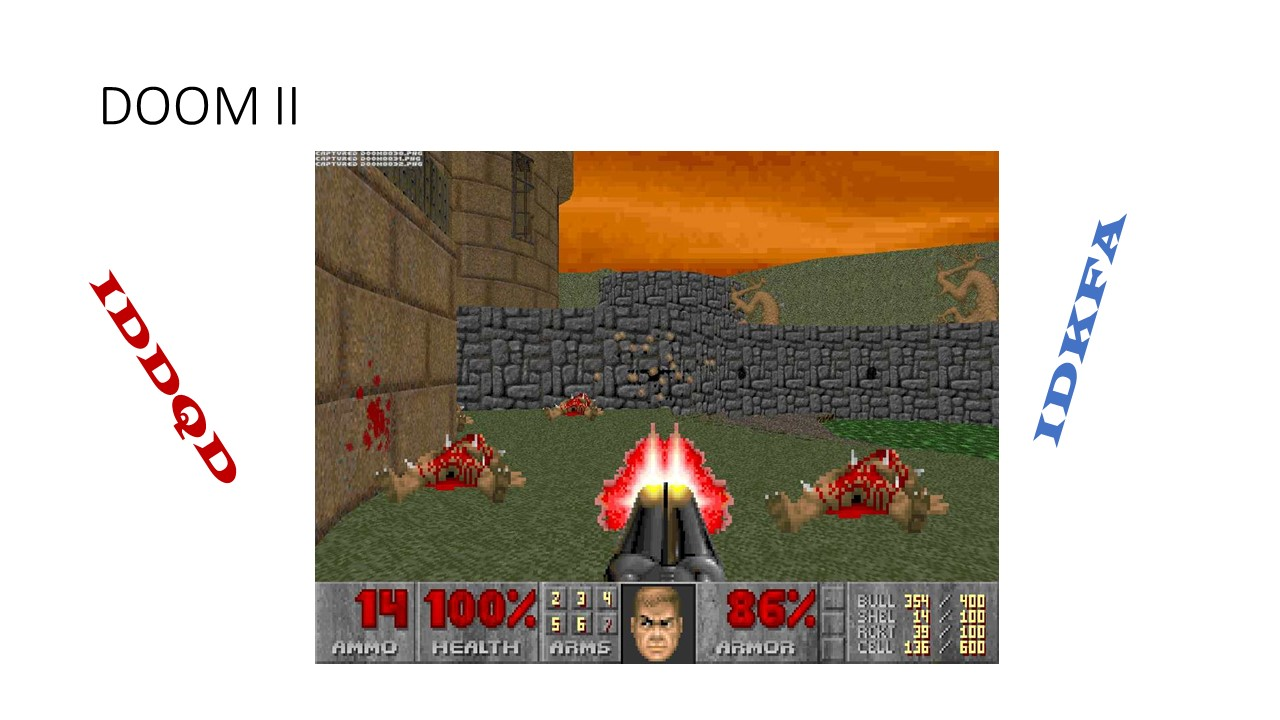
\includegraphics[width=\textwidth]{advert/slide5.jpg}
	\end{frame}
		
	\begin{frame}
		\centering
		\huge{Интеллектуальное планирование и когнитивные архитектуры}
		\par\bigskip
		\large{Константин Яковлев, Александр Панов}
		\par\bigskip
		\Large{Базовая кафедра\\
			<<Математические методы системного анализа>>\\
			Института системного анализа РАН\\
			\url{www.cs.hse.ru/mmsa}
		}
	\end{frame}
			
	\begin{frame}
		\frametitle{Кратко о себе}
		\scriptsize
		\begin{columns}
			\begin{column}{0.85\textwidth}
				\textbf{Панов Александр Игоревич, к. ф.-м. н.}
				\begin{itemize}
					\item Научный сотрудник лаборатории <<Динамические интеллектуальные системы>> Института системного анализа Федерального исследовательского центра <<Информатика и управление>> Российской академии наук.
					\item Научный сотрудник и старший преподаватель в Высшей школе экономики.
					\item Ассистент в Московском физико-техническом институте.
					\item Член редколлегии журнала Biologically Inspired Cognitive Architectures (BICA Journal).
					\item Член Российской ассоциации искусственного интеллекта (РААИ).
					\item Член Сообщества биологически инспирированных когнитивных архитектур (BICA Society).
					\item Организатор Международной	школы по биологически инспирированным когнитивным архитектурам (Fierces on BICA, Москва) и Международной конференции по биологически инспирированным когнитивным архитектурам (BICA-2016, Нью-Йорк).
					\item Член рабочей группы <<Нейронет>> Национальной технологической инициативы.
					\item Руководитель проектов РФФИ мол\_а и мол\_а\_дк.
				\end{itemize}
			\end{column}
			
			\begin{column}{0.15\textwidth}
				\centering
				
\includegraphics[width=\textwidth]{advert/ras.png}
				\vspace{7pt}
				
\includegraphics[width=0.7\textwidth]{advert/isa.png}
				\vspace{7pt}
				
\includegraphics[width=0.5\textwidth]{advert/raai.png}
				\vspace{7pt}
				
\includegraphics[width=0.5\textwidth]{advert/hse.png}
				\vspace{7pt}
				
\includegraphics[width=\textwidth]{advert/mipt.jpg}
				\vspace{7pt}
				
\includegraphics[width=\textwidth]{advert/bica2016.png}
				\vspace{7pt}
				
\includegraphics[width=0.7\textwidth]{advert/nti.jpg}
			\end{column}
			
		\end{columns}
	\end{frame}

	\begin{frame}
		\frametitle{Кратко о себе}
		\scriptsize
		\begin{columns}
			\begin{column}{0.85\textwidth}
				\textbf{Яковлев Константин Сергеевич, к. ф.-м. н.}
				\begin{itemize}
					\item Старший научный сотрудник лаборатории <<Динамические интеллектуальные системы>> Института системного анализа Федерального исследовательского центра <<Информатика и управление>> Российской академии наук.
					\item Старший преподаватель Высшей школы экономики (факультет компьютерных наук).
					\item Доцент Российского университета дружбы народов (факультет физико-математических и естественных наук).
					\item Член Российской ассоциации искусственного интеллекта (РААИ).
					\item Организатор ежегодного всероссийского семинара <<Беспилотные транспортные средства с элементами искусственного интеллекта>> (БТС-ИИ)
					\item Финалист конкурса летающих роботов (КРОК-2013).
					\item Член рабочей группы <<Аэронет>> Национальной технологической инициативы.
					\item Руководитель проектов РФФИ а и мол\_а\_вед.
				\end{itemize}
			\end{column}
			
			\begin{column}{0.15\textwidth}
				\centering
				
\includegraphics[width=\textwidth]{advert/ras.png}
				\vspace{7pt}
				
\includegraphics[width=0.7\textwidth]{advert/isa.png}
				\vspace{7pt}
				
\includegraphics[width=0.5\textwidth]{advert/raai.png}
				\vspace{7pt}
				
\includegraphics[width=0.5\textwidth]{advert/hse.png}
				\vspace{7pt}
				
\includegraphics[width=0.5\textwidth]{advert/rupf.png}
				\vspace{7pt}
				
\includegraphics[width=0.5\textwidth]{advert/aiuv.png}
				\vspace{7pt}
				
\includegraphics[width=0.5\textwidth]{advert/aeronet.png}
			\end{column}
		\end{columns}
	\end{frame}
	
	\begin{frame}
		\frametitle{Научные интересы}
		\begin{itemize}
			\item \textit{Искусственный интеллект}: интеллектуальные системы управления, интеллектуальные динамические системы, робототехника, автоматическое планирование, эвристический поиск.
			\item \textit{Когнитивное компьютерное моделирование}: планирование поведения, модели внимания, восприятия, принятия решений и обучения, знаковые системы.
			\item \textit{Многоагентные системы}: когнитивные агенты, образование коалиций, распределение ролей в коллективе, целеполагание.
			\item \textit{Анализ данных}: выявление причинно-следственных связей, анализ психологических и медицинских данных.
			\item \textit{Распознавание изображение}: выявление объектов на сложных сценах, рекуррентные и глубокие нейронные сети.
			\item \textit{Системы управления}: управление поведением, многоуровневые архитектуры, робототехника.
		\end{itemize}
	\end{frame}
	
	\begin{frame}
		\frametitle{Программа курса}
		
		\begin{itemize}
			\tiny 
			\item<pro@1-> Введение: что такое когнитивные архитектуры (КА) и зачем они нужны. Обзор существующих КА и их функциональных особенностей.
			\item<pro@1-> Основные КА: Soar.
			\item<pro@1-> Основные КА: ACT-R (практическая задача \textnumero 1).
			\item<con@1-> Основные КА: STRL.
			\item<pro@1-> Основные КА: ACT-R (прием задания \textnumero 1).
			\item<con@1-> Функции КА: планирование. Методы решения задачи планирования.
			\item<pro@1-> Функции КА: память и обучение. Модели представление знаний и их пополнения.
			\item<con@1-> Планирование поведения I (STRIPS) (практическая задача \textnumero 2).
			\item<pro@1-> Память и обучение: рекуррентные нейронные сети.
			\item<con@1-> Планирование поведения I (STRIPS) (прием задания \textnumero 2).
			\item<pro@1-> Память и обучение: неокогнитрон (практическая задача \textnumero 3).
			\item<con@1-> Планирование поведения II (Graphplan).
			\item<con@1-> Планирование поведения II (Graphplan).
			\item<pro@1-> Память и обучение: неокогнитрон (прием задания \textnumero 3).
			\item<con@1-> Планирование поведения III (HTN).
			\item<con@1-> Робототехника: планирование траекторий (LIAN) (практическая задача \textnumero 4).
			\item<pro@1-> Память и обучение: иерархическая временная память.
			\item<con@1-> Планирование поведения III (LIAN) (прием задания \textnumero 4).
			\item<pro@1-> Психологически правдоподобные модели в КА. Знаковая картина мира.
		\end{itemize}
		
		4 практических задачи --- полное и своевременное выполнение --- автоматы. Для остальных в конце --- письменный экзамен.
		
		3-4 модули 3 курса.
	\end{frame}

	\begin{frame}
		\frametitle{Когнитивные архитектуры}
		
		\begin{columns}
			\begin{column}{0.5\textwidth}
				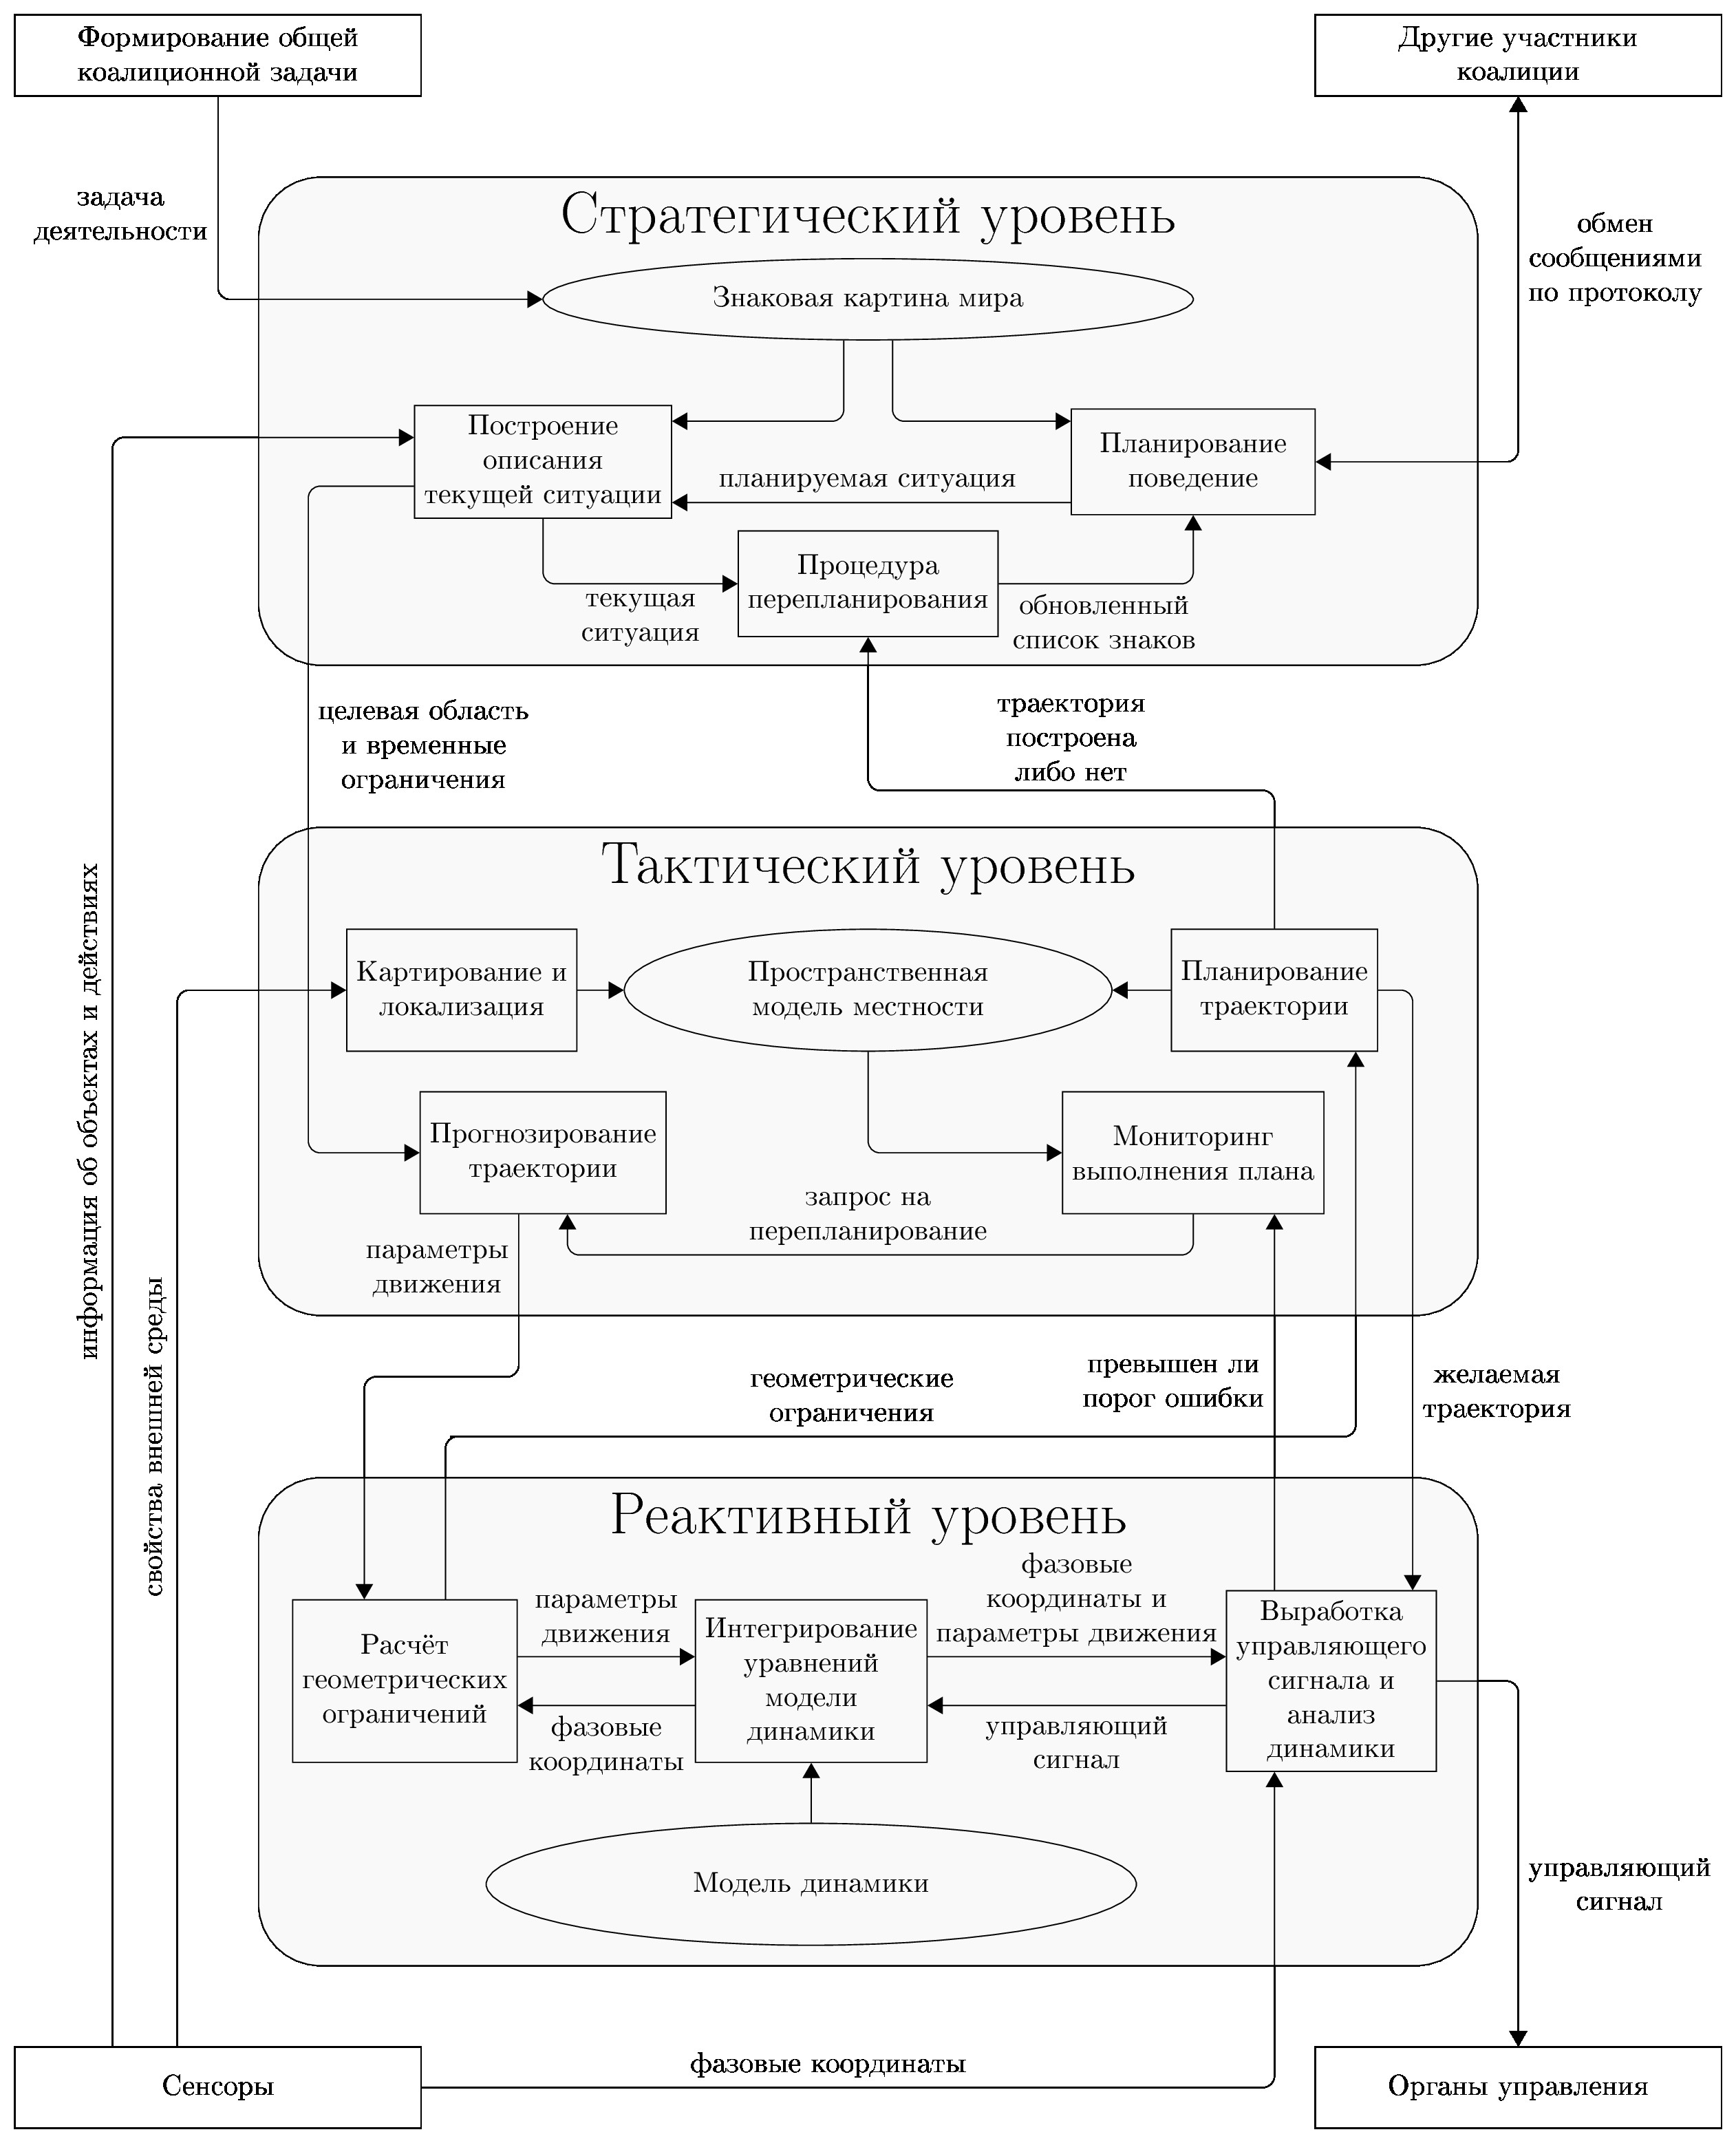
\includegraphics[width=0.9\textwidth]{strl/architecture}
			\end{column}
			\begin{column}{0.5\textwidth}
				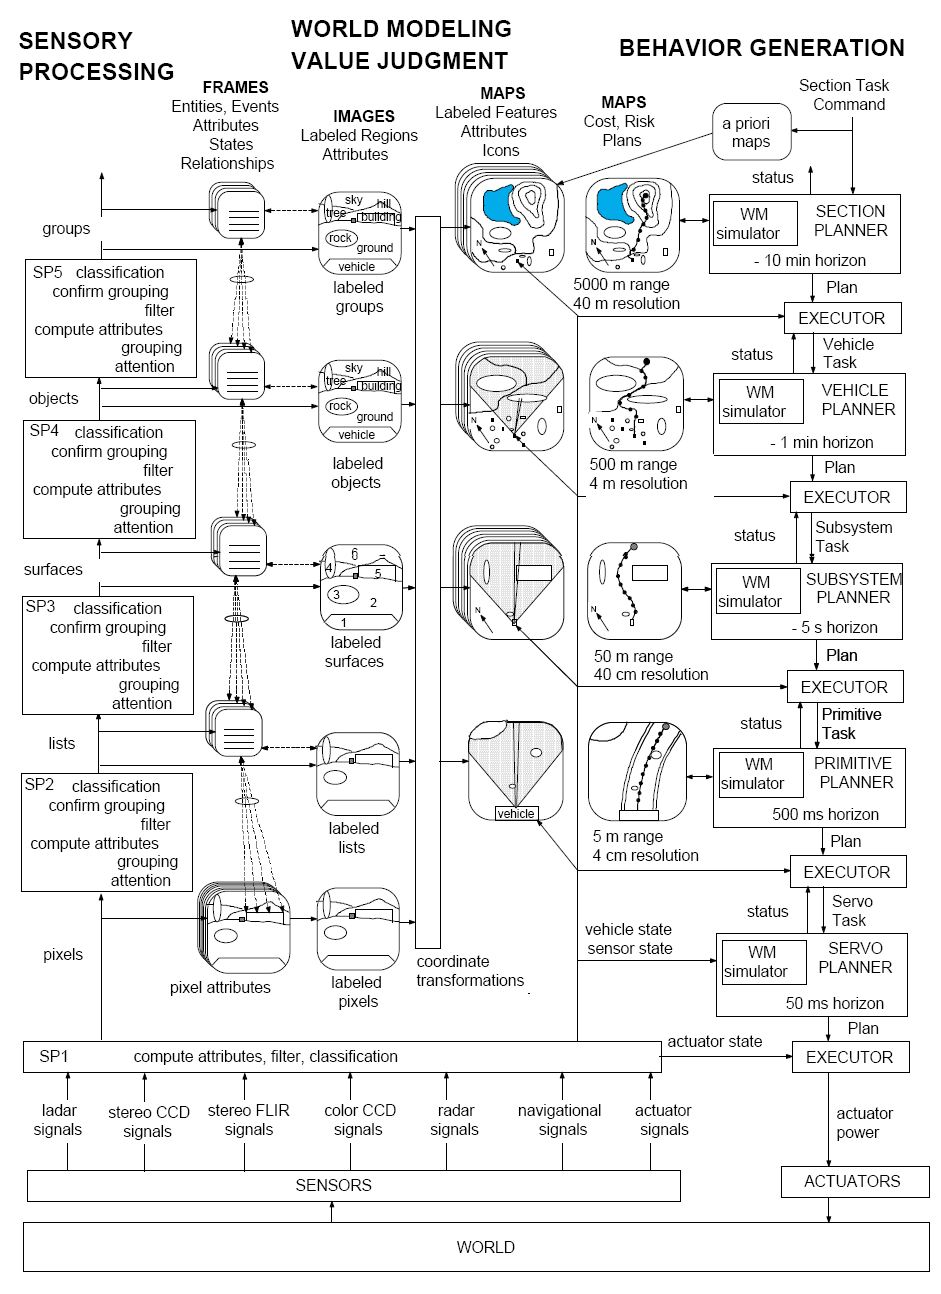
\includegraphics[width=0.8\textwidth]{strl/4d-rcs}
			\end{column}			
		\end{columns}
	\end{frame}
	
	\begin{frame}
		\frametitle{Как устроен мозг}
		
		\begin{columns}
			\begin{column}{0.3\textwidth}
				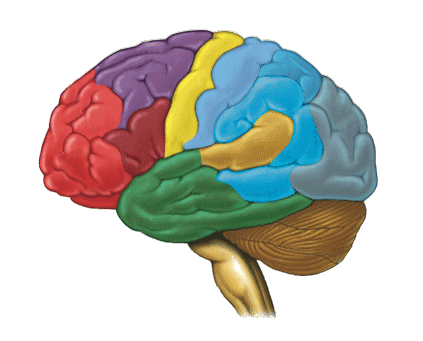
\includegraphics[width=0.9\textwidth]{phisio/mozg_2}
				\par\bigskip
				\hspace{-7mm}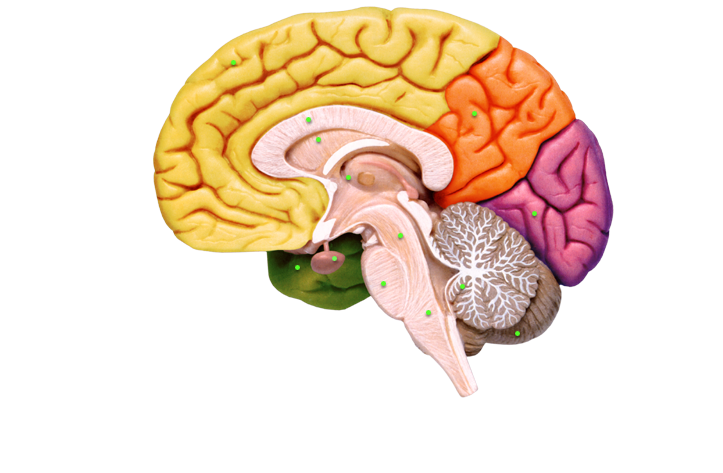
\includegraphics[width=1.1\textwidth]{phisio/mozg}
			\end{column}
			\begin{column}{0.4\textwidth}
				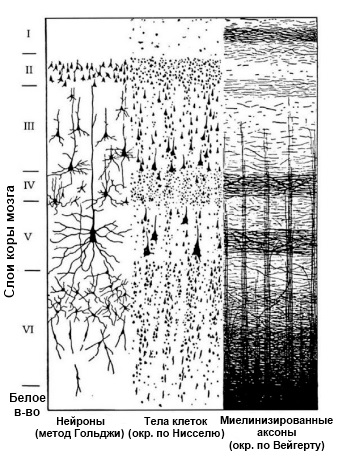
\includegraphics[width=0.9\textwidth]{phisio/column_layers_ru}
			\end{column}
			\begin{column}{0.3\textwidth}
				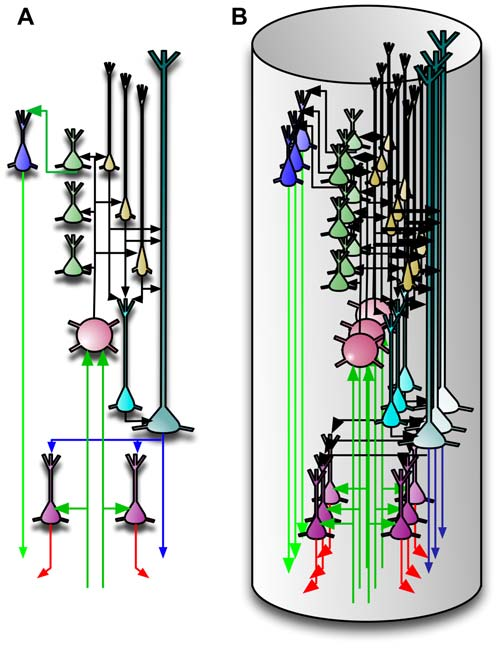
\includegraphics[width=\textwidth]{phisio/column}
			\end{column}			
		\end{columns}
	\end{frame}
	
	\begin{frame}
		\frametitle{Символьные вычисления}
		
		\begin{columns}
			\begin{column}{0.5\textwidth}
				\centering
				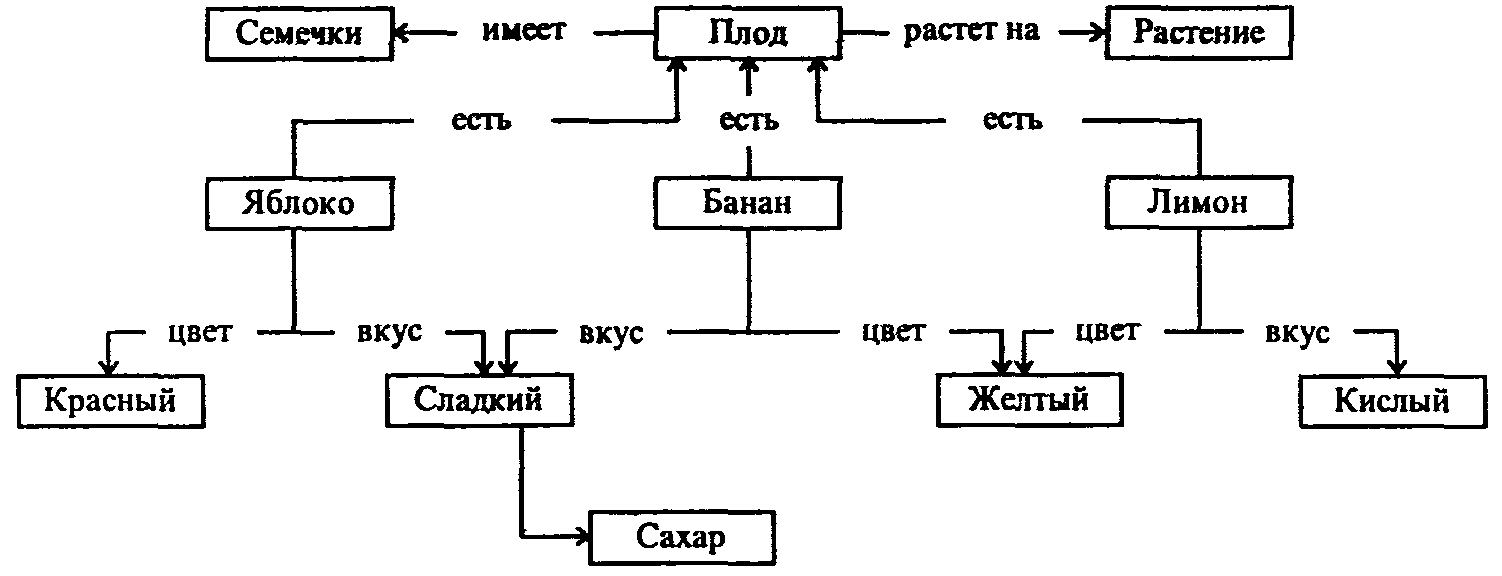
\includegraphics[width=\textwidth]{advert/semnet1}
				\par\bigskip
				\hspace{-7mm}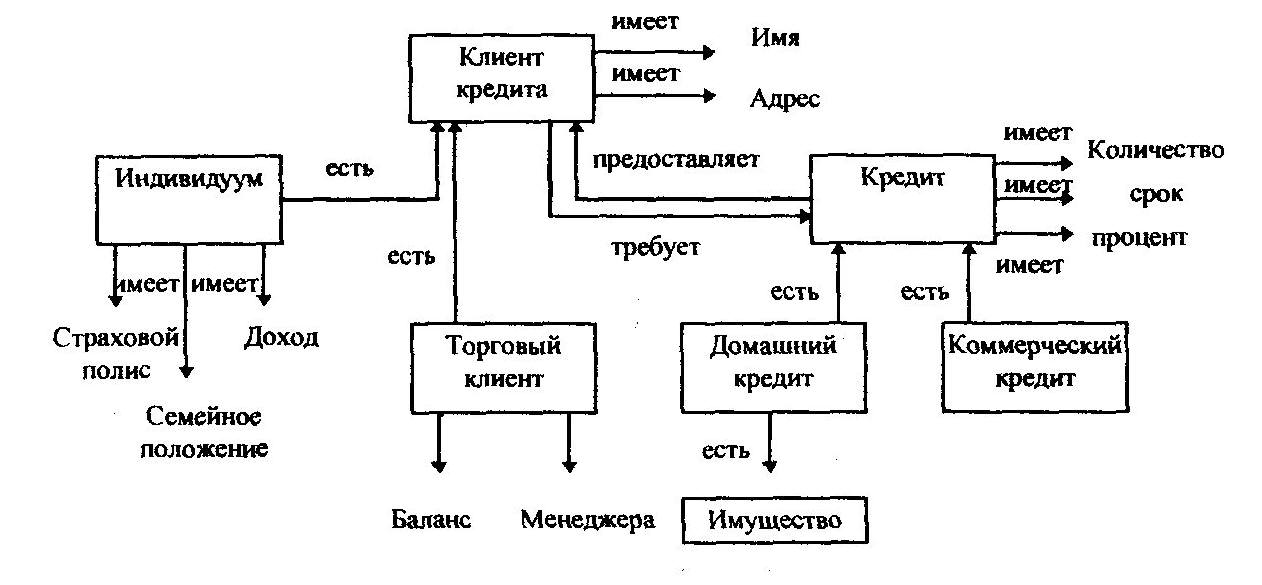
\includegraphics[width=\textwidth]{advert/semnet2}
			\end{column}
			\begin{column}{0.5\textwidth}
				\centering
				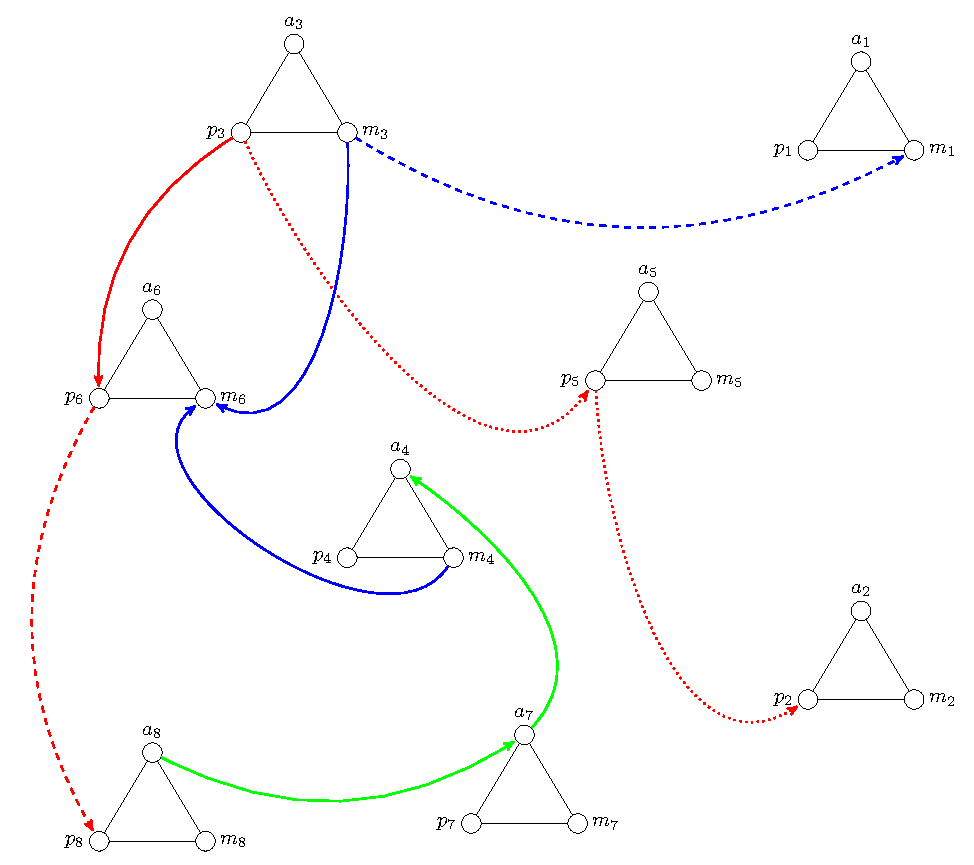
\includegraphics[width=0.8\textwidth]{signs/signs_net}
				\par\bigskip
				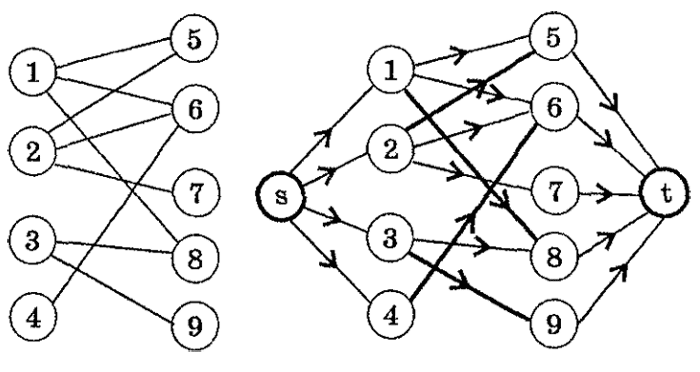
\includegraphics[width=0.7\textwidth]{advert/graph}
			\end{column}			
		\end{columns}
	\end{frame}

	\begin{frame}
		\frametitle{Стажировки в научном институте}
		
		Лето 2016 года.
		\par\bigskip
		\begin{itemize}
			\item Работа над реальным научным проектом.
			\item Опыт работы в передовой научной лаборатории.
			\item Опыт программирования интересных задач.
			\item \textbf{Оплачиваемое удовлетворение собственного любопытства.}
		\end{itemize}
	\end{frame}
	
	\begin{frame}
		\centering
		\Huge
		Спасибо за внимание!
		\normalsize
		\par\bigskip
		\par\bigskip
		Базовая кафедра\\
		<<Математические методы системного анализа>>\\
		Института системного анализа РАН
		\par\bigskip
		\par\bigskip
		apanov@hse.ru, kyakovlev@hse.ru
	\end{frame}
														
%	\begin{frame}
%		\frametitle{Цели курса}
%		
%		\begin{columns}
%			\begin{column}{0.5\textwidth}
%				
%			\end{column}
%			\begin{column}{0.5\textwidth}
%				\begin{figure}
%					
\includegraphics[width=\textwidth]{logo}
%				\end{figure}
%			\end{column}
%		\end{columns}
%	\end{frame}
	%	\begin{frame}
	%		\frametitle{Цели курса}
	%		
	%		\begin{itemize}
	%			\item
	%		\end{itemize}
	%	\end{frame}
	
\end{document}
	
	
